\documentclass[]{subfiles}

\begin{document}
\section{Anforderungen}
    Im folgenden Abschnitt werden die Anforderungen an ein Netzwerk-Test-System formuliert.
    Es werden die Kern-Akteuere identifiziert und deren Funktion und Abhängigkeiten 
    und Anforderungen formuliert, um auf dieser Basis die Software zu entwerfen.
    
    \subsection{Akteure in einem Netzwerksystem}
    In der Praxis gibt es für die verschiedenen Akteure in einem Netzwerksystem
    unterschiedliche Bezeichnungen. Beispielsweise ist oft nicht klar, was der 
    Unterschied zwischen einem Netzwerk-Architekten und einem Netzwerk-Engineer
    ist und welche Verantwortungen diese nun genau haben. Wir haben eine eigene
    Unterscheidung der Akteure formuliert und diese in den kommenden Sektionen
    dokumentiert, um eine einheitliche Basis für die Leser zu schaffen.

    \subsubsection*{Netzwerk-Architekt}
    Ein Netzwerk-Architekt plant und erstellt Kommunikationsnetzwerke.
    Im Zuge dieser Arbeit wurde zwischen dem Architekten als verantwortlichen
    Senior-Network-Engineer und einem Network Engineer (Junior oder Senior)
    als operativen Mitarbeiter unterschieden. 
    Der Architekt nimmt dabei eher die Rolle des Managers oder Teamleiters ein. 
    Er führt dabei normalerweise keine Konfigurationen am Netzwerk durch.

    \subsubsection*{Netzwerk-Engineer}
    Ein Netzwerk-Engineer ist für die Installation und Instandhaltung 
    eines Netzwerks zuständig. 
    Er ist dem Netzwerk-Architekten unterstellt und setzt mit Ihm
    zusammen die geplanten Arbeiten um. 

    \subsubsection*{Netzwerk-Administrator}
    Der Netzwerk Administrator hat üblicherweise eine abgeschlossene Berufslehre 
    in der Informatik und arbeitet zusammen mit dem Netzwerk-Engineer am Netzwerk. 
    Es wird davon ausgegangen, dass ein Netzwerk Administrator keine bis wenige 
    Programmierkenntnisse hat. 
    Ein Netzwerk Administrator hat, je nach Grösse des Netzwerks, 
    nur Kenntnisse über einen Teil der Netzwerkumgebung. 
    Er führt dabei ihm vom Architekten oder Engineer vorgegebene Arbeiten 
    aus und muss dazu nicht den vollen Überblick über das Netzwerk und die 
    darin verwendeten Technologien haben.

    \subsubsection*{Netzwerk-User}
    Benutzer der Netzwerkumgebung. User können das Netzwerk verwenden,
    aber nicht dessen Konfigurationen anpassen.


    \subsubsection*{Netzwerk-Gerät}
    Ein Netzwerkgerät kann aus Hardware wie Switch, Router oder Server
    bestehen oder Virtuell als Software implementiert sein. 
    Im Zuge der Arbeit werden Netzwerkgeräte auch als Netzwerk-Devices 
    oder einfach Device bezeichnet. 
    Typischerweise haben Devices eine Statische Konfiguration und einen 
    dynamischen Zustand zur Laufzeit. 
    In den kommenden Kapiteln wird genauer auf Netzwerkgeräte eingegangen.

    \subsubsection*{Netzwerk-Verbindung}
    Die Netzwerkverbindung ist der Kommunikationskanal zwischen den einzelnen
    Netzwerkgeräten. Sie kann in physischer Form als Kabel, oder mit kabellosen
    Mitteln z.B. Funk umgesetzt sein. Die Wahl des Übertragungsmediums hat
    grossen Einfluss über die verfügbare Bandbreite und mögliche Störfaktoren.

    \subsubsection*{Repository/Inventar}
    Im Inventar werden die Unterschiedlichen Devices mit den für den 
    Betrieb wichtigsten Parametern gespeichert. 
    Das Inventar kann in digitaler Form als Repository, 
    als File auf einem Ordner/Computer, 
    oder analogin einem Dokumentenorder abgelegt sein. 
    Das Inventar wird benötigt, um die aktuellen Konfigurationen, 
    die physische Position des Geräts oder sonstige für den Betrieb 
    relevanten Informationen zu dokumentieren.

    \newpage

    \subsection{Akteure in der zu entwickelnden Software}

    \subsubsection*{Testprogramm}
    Das Testprogramm ist der Kern des zu entwickelnden Systems dieser Arbeit.
    Es Interagiert mit den anderen Akteuren und hat, vom Akteur und Kontext abhängig, 
    unterschiedliche Anforderungen.
    Es soll so aufgebaut sein, dass ein Benutzer der Software diese mit möglichst 
    geringem Aufwand bedienen kann.


    \subsubsection*{Testdefinitionssprache}
    Wird im Rahmen dieser Arbeit auch als Testbeschreibungssprache oder Definitionssprache
    bezeichnet. Eine Testdefinition beschreibt die einzelnen Testfälle, die von einem
    System durchgeführt werden sollen.
    Die Definitionssprache soll dabei in einem Format gehalten werden, das von 
    allen Benutzern der Software verstanden wird und von diesen erweitert werden kann.

    \subsubsection*{Testreport}
    Ein Testreport soll, möglichst einfach und genau, die Ergebnisse eines 
    Netzwerktests aufzeigen. 
    Fehlgeschlagene Tests sollen dabei möglichst einfach und schnell zu erkennen
    sein und alle Informationen beinhalten, die ein Betrachter benötigt, um
    den Fehler im System zu lokalisieren und beheben.
    Ausserdem muss mindestens noch ein Zeitstempel vorhanden sein, um die
    Historie vergangener Netzwerktests nachvolziehen zu können.
    Testreporte können auf dem System, welches die Tests ausführt, oder in 
    einem zentralen Repository abgelegt werden, damit mehrere Mitglieder eines 
    Netzwerkteams gleichzeitig darauf zugreifen können.     

    \subsubsection*{Kommunikationskanal}
    Der Kommunikationskanal, nicht zu verwechseln mit der Netzwerkverbindung zwischen
    zwei Netzwerkgeräten, verbindet ein zu testendes Netzwerk mit dem Testprogramm.
    Möglichkeiten für einen Kanal sind beispielsweise das SSH (secure shell) Protokoll
    oder der Restconf Standard.
    Dies kann über eine Kabelverbindung oder Kabellos geschehen.
    Die Wahl des Kommunikationskanals beeinflusst dabei, in welcher Form 
    Netzwerktests durchgeführt werden können und in welchem Format die Ergebnisse 
    zurückgegeben werden.

    \subsubsection*{Netzwerktest}
    Werden heute meist manuell oder mit Hilfe eines Skripts durchgeführt.
    Ein automatisierter Netzwerktest sollte hypothetisch ad-hoc nach jeder
    Konfigurationsänderung vom Testprogramm durchgeführt werden um 
    die Funktionsweise des Netzwerks zu validieren. 
    Ein Benutzer des zu entwickelnden Systems soll in der Lage sein, 
    mit nur geringer Einarbeitungszeit, Netzwerktests zu spezifizieren und
    durchzuführen.

    \newpage

    \subsection{Use Cases}
    \subsubsection{Use Case Diagramm}
    \begin{figure}[!h] 
        \centering
        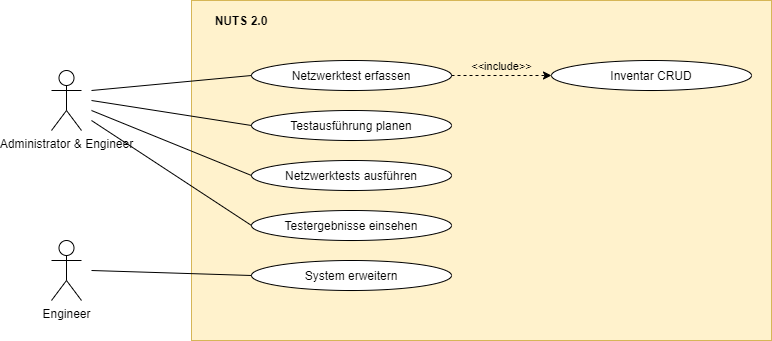
\includegraphics[scale=0.5]{../../99_Vorlagen/Bilder/UseCaseDiagram.png}
        \caption{Use Case Diagramm}
    \end{figure}
    \subsubsection{Aktoren}
    Die Primären Akteure sind der Netzwerk Architekt, -Administrator und -Engineer. 
    Der Architekt will primär die Ergebnisse einsehen können, um zu sehen, dass
    das Netzwerk korrekt funktioniert. 
    Ausserdem möchte er, beispielsweise um eine Erweiterung des Netzwerks zu 
    Planen, eine Ausführung von Netzwerktests konfigurieren und durchführen.
    Der Administrator will Netzwerktests erfassen, deren Durchführung planen, 
    die Tests durchführen und die Ergebnisse einsehen.
    Der Engineer möchte neben den Tätigkeiten, die der Administrator ausführt,
    zudem das Testsystem um weitere Netzwerktests erweitern können.

    \subsection{Beschreibung Usecases (Brief)}

        \paragraph{Netzwerktest erfassen}
        Ein Netzwerktest setzt sich zusammen aus der Testdefinition mit den zu testenden Devices, 
        Befehle, die auf den Devicesv ausgeführt werden sollen, einem oder mehreren 
        Kommunikationskanälen, über den die Devices angesprochen werden
        und einem Erwartungswert für das Ergebnis. 
        Diese Informationen werden in einer Testdefinitionssprache gespeichert, 
        welche so strukturiert sein muss, dass sie ein Softwaresystem einfach laden 
        kann und trotzdem von Menschen interpretiert werden kann. 
        Die Erfassung eines Netzwerktests soll so einfach wie möglich gehalten werden, 
        damit Administratoren und Engineers effizient neue Tests spezifizieren können.

        \paragraph{Inventar CRUD}
        Der Netzwerk Engineer oder -Administrator möchte die physischen und virtuellen 
        Netzwerkgeräte und deren statische Konfiguration in einem Inventar verwalten.
        Das Inventar wird von dem zu entwickelnden System verwendet, um die 
        Gerätekonfigurationen wie z.B. Zugangsdaten oder Herstellerinformationen abzurufen.
        Es soll möglich sein, das Inventar automatisiert zu erstellen und Geräte in distinkte
        Gruppen zu kategorisieren. 

        \paragraph{Testdurchführung planen}
        Themen, die in der Testausführung relevant sind, sind die Auswahl, 
        welche Tests überhaupt ausgeführt werden sollen, die Reihenfolge der Tests, 
        auf welchen Teil des Systems sie angewandt werden sollen 
        und ob sie synchron oder asynchron durchgeführt werden. 
        Weitere Punkte wären das automatische durchführen von Tests zu spezifischen 
        Zeiten oder Wochentagen und dass die Testkonfiguration gespeichert wird, 
        um sie später anzupassen. 
        Auch hier ist darauf zu achten, dass das zu entwickelnde System so aufgebaut ist, 
        dass Engineers, Architekten und Administratoren effizient arbeiten können.

        \paragraph{Netzwerktests durchführen}
        Der Anwender möchte die in der Testdurchführung geplanten Netwerktests auf das
        angegebene System ausführen. 
        Dazu wird in einer Benutzeroberfläche die Testausführung gestartet oder auf
        einem Gerät automatisch die zu entwickelnde Software ausgeführt.

        \paragraph{Testergebnisse einsehen}
        Nachdem ein Test durchgeführt wurde, soll ein Testresultat angezeigt werden. 
        In den Resultaten soll ersichtlich sein, welche Tests durchgeführt wurde, 
        was der Test genau gemacht hat, welche Befehle auf welchen Devices ausgeführt 
        wurde und wie das Ergebnis ist. 
        Die Testergebnisse sollen auf der Konsole/Benutzeroberfläche ersichtlich sein 
        und zusätzlich in einem Testreport mit Datum und Uhrzeit gespeichert werden, 
        damit die Historie des Netzwerks ermittelt werden kann. 
        Wenn Tests durch einen Fehler im zu entwickelnden System nicht durchgeführt 
        werden kann, sollen alle anderen Tests nicht davon beeinflusst werden und 
        das Ergebnis soll einen Vermerk für das Versagen des Systems beinhalten,
        mit dem der Anwender in der Lage ist, die Ursache zu ermitteln und zu beheben.

        \paragraph{System erweitern}
        Engineers sollen in der Lage sein, das System bei Bedarf zu erweitern, 
        z.B. um weitere Tests oder Netzwerkschnittstellen hinzuzufügen oder 
        Fehler zu verbessern. 
        Die Erweiterungen beschränken sich aber auf rein funktionale Bereiche des Systems. 
        Für Änderungen an der Benutzeroberfläche sollen Softwareengineers mit 
        Erfahrung auf dem Gebiet hinzugezogen werden.

    \newpage

    \subsection{Nichtfunktionale Anforderungen}
    In diesem Kapitel werden die nichtfunktionalen Anforderungen an das Projekt behandelt.
    Es werden Aspekte und Anforderungen aus den Bereichen Änderbarkeit, Benutzbarkeit, 
    Effizienz, Zuverlässigkeit, Betreibbarkeit und Sicherheit gemäss ISO/IEC 9126 betrachtet.
	Die jeweiligen Aspekte werden in ihren Unterkapiteln genauer beschrieben.
    Es wurden mögliche Szenarien erarbeitet, die in der Erstellung oder dem Betrieb 
    der Software auftreten können und beim Architekturdesign in betracht gezogen wurden.

	\subsubsection{Änderbarkeit}
		Aufwand, der zur Durchführung von vorgegebenen Änderungsarbeiten benötigt wird.
		Unter Änderungen gehen Korrekturen, Anpassungen oder Veränderungen der Umgebung, Anforderungen oder funktionalen Spezifikation.
		Gemäss ISO 9126 gehören zur Änderbarkeit folgende Teilmerkmale:
		
		\paragraph{Analysierbarkeit}
			Aufwand, der benötigt wird, um das System zu verstehen, z.B. um Ursachen von Versagen oder Mängel zu diagnostizieren oder Änderungen zu planen.

		\paragraph{Modifizierbarkeit}
			Wie leicht lässt sich das System anpassen, um Verbesserungen oder Fehlerbeseitigungen durchzuführen.

		\paragraph{Stabilität}
			Wahrscheinlichkeit, dass mit Änderungen unerwartete Nebenwirkungen auftreten.

		\paragraph{Testbarkeit}
			Wie gross wird der Aufwand, bei Änderungen die Software zu prüfen.

		\newpage

		\paragraph{Szenario: Neue Netzwerkschnittstelle}
			Wenn zum bestehenden System eine neue Netzwerkschnittstelle definiert werden soll, so muss die dafür notwendige Software innerhalb von einer Arbeitswoche entwickelt, integriert und in Betrieb genommen werden können.
			
			\begin{table}[!h]
				\begin{tabularx}{\textwidth}{lX}
					\toprule
					Qualitätsziele & Flexibilität, Erweiterbarkeit, Anpassbarkeit, Austauschbarkeit  \\
					\midrule
					Geschäftsziel(e) & Software kann mit geringem Aufwand an geänderte Anforderungen angepasst werden  \\
					\midrule
					Auslöser & Ein Engineer möchte weitere Tests einbinden oder Schnittstellen, die nicht im System integriert sind.  \\
					\midrule
					Reaktion & Die Software lässt sich von einem Entwickler in weniger als einer Woche um benötigte Komponenten erweitern.  \\
					\midrule
					Zielwert & 	Erweiterungen der Netzwerkschnittstellen oder Anpassungen von Tests sind innerhalb von 40 Personenstunden umsetzbar.  \\
					\bottomrule
				\end{tabularx}
				\caption{Szenario: Neue Schnittstelle}
			\end{table}
			

		\paragraph{Scenario: Schnelle Fehlerlokalisierung}
			Die Ursache von fehlgeschlagenen Tests (Software-Unittests) lässt sich in kurzer Zeit lokalisieren.
			
			\begin{table}[!h]
				\begin{tabularx}{\textwidth}{lX}
					\toprule
					Qualitätsziele & Schnelle Fehlerbehebung, Änderbarkeit, Anpassbarkeit, geringes Risiko bei Erweiterungen  \\
					\midrule
					Geschäftsziel(e) & Entwickler können das Programm einfach anpassen und erkennen im Fehlerfall schnell, was nicht funktioniert hat.  \\
					\midrule
					Auslöser & Eine Änderung im Code führt zu Fehlnern in der Ausführung.  \\
					\midrule
					Reaktion & Wenn ein Fehler dazu führt, dass die Softwareausführung fehlschlägt, kann ein Entwickler aufgrund von Fehler- und/oder Log-Nachrichten die Ursache in kurzer Zeit lokalisieren.  \\
					\midrule
					Zielwert & Fehlerlokalisierung findet durchschnittlich in weniger als 10 Minuten statt.  \\
					\bottomrule
				\end{tabularx}
				\caption{Szenario: Schnelle Fehlerlokalisierung}
			\end{table}
			
			\newpage

	\subsubsection{Benutzbarkeit}
		Zeitlicher Aufwand, der für die Erlernung der Benutzung des Programms benötigt wird. 
		Die User werden hierfür in spezifische Nutzergruppen mit festgelegten Fähigkeiten unterteilt.
		
		\paragraph{Verständlichkeit}
			Aufwand für den Nutzer, die Konzepte und Menüführung der Anwendung zu verstehen.

		\paragraph{Erlernbarkeit}
			Aufwand für den User, sich ohne Vorwissen in das System einzuarbeiten.

		\paragraph{Bedienbarkeit}
			Aufwand für den Benutzer, die Anwendung zu bedienen.

		\paragraph{Szenario: Einfachheit der Definitionssprache}
			Die Definitionen von Inventar und Tests sind so aufgebaut, dass ein User in kurzer Zeit die Struktur und den Aufbau versteht und eigene Tests implementieren kann.
			
			\begin{table}[!h]
				\begin{tabularx}{\textwidth}{lX}
					\toprule
					Qualitätsziele & Produktivität, Einfachheit, Verständlichkeit \\
					\midrule
					Geschäftsziel(e) & Einarbeitung in die Testdefinition erfolg möglichst einfach und benötigt nur geringes Vorwissen.  \\
					\midrule
					Auslöser & Ein Nutzer, welcher keine Erfahrung im Umgang mit der Software hat, möchte eigene Tests definieren.  \\
					\midrule
					Reaktion & Benutzer können sich schnell in die Testdefinitionen einlesen und rasch eigene Tests definieren, vorausgesetzt, sie haben Kenntnisse des Netzwerkes.  \\
					\midrule
					Zielwert & Ungeschulte Nutzer verstehen innerhalb von durchschnittlich 30 Minuten die Struktur und den Aufbau der Testdefinitionen und sind in der Lage, eigene Tests zu erstellen.  \\
					\bottomrule
				\end{tabularx}
				\caption{Szenario: Einfachheit der Definitionssprache}
			\end{table}
			\newpage
			
		\paragraph{Szenario: Hinweis auf Fehleingaben}
		Fehlerhafte Eingaben werden vom System ignoriert und der Benutzer wird auf die falsche Eingabe hingewiesen. Das Programm führt fehlerfreie Programmteile unabhängig von den Fehlern durch.
		
		\begin{table}[!h]
			\begin{tabularx}{\textwidth}{lX}
				\toprule
				Qualitätsziele & Robustheit, Verständlichkeit, Fehlertoleranz.  \\
				\midrule
				Geschäftsziel(e) & Fehleingaben führen nicht dazu, dass die Tests nicht mehr durchgeführt werden können.  \\
				\midrule
				Auslöser & Ein Benutzer macht einen Fehler bei der Testdefinition und startet das Programm.  \\
				\midrule
				Reaktion & Das Programm führt alle korrekten Tests durch und informiert den Benutzer, dass es fehlerhafte Tests gibt, die nicht durchgeführt werden können. Die Hinweise werden im Report und auf der Konsolenausgabe geschrieben.   \\
				\midrule
				Zielwert & Tests sind einzeln gekapselt und werden unabhängig voneinander durchgeführt. Falscheingaben werden vom Programm detektiert und im Testreport sowie auf der Konsolenausgabe erwähnt.  \\
				\bottomrule
			\end{tabularx}
			\caption{Szenario: Hinweis auf Fehleingaben}
		\end{table}
		
		
	\subsubsection{Effizienz}
	Mit Effizienz ist die 'performance efficiency' gemeint, d.h. das Verhältnis zwischen dem Leistungsniveau der Software und den eingesetzten Hardwarekomponenten. 
	Andere Beschreibungen umfassen: Skalierbarkeit, Speicherbedarf, Verarbeitungsgeschwindigkeit, Antwortzeit etc.
	Teilmerkmale nach ISO 9126:

		\paragraph{Zeitverhalten}
		Dauer für Verarbeitung und Antwortzeit sowie Durchsatz bei der Ausführung des Programms

		\paragraph{Verbrauchsverhalten}
		Wie viel Speicherbedarf hat das Programm, wie lange werden Betriebsmittel in Anspruch genommen und welche Hardwarekomponenten werden benötigt.

	\subsubsection{Zuverlässigkeit}
	Unter Zuverlässigkeit versteht man die Fähigkeit der Software, unter festgelegten Bedingungen die Funktionalität über einen definierten Zeitraum zu gewährleisten
	
		\paragraph{Reife}
		Geringe Ausfallhäufigkeit durch Fehlzustände.

		\paragraph{Fehlertoleranz}
		Die Software ist in der Lage, trotz Fehlern ihr spezifiziertes Leistungsniveau beizubehalten.

		\paragraph{Wiederherstellbarkeit}
		Im Fehlerfall können betroffene Daten wiederhergestellt und die Funktionalität wieder aufgenommen werden.

		\paragraph{Szenario: Tests lassen sich auf der Netzwerkseite nicht ausführen}
		Falls ein Test auf dem jeweiligen Netzwerkgerät nicht erfolgreich durchgeführt werden kann, läuft das Programm weiter und definiert den dazugehörigen Netzwerktest als nicht bestanden.
		
		\begin{table}[!h]
			\begin{tabularx}{\textwidth}{lX}
				\toprule
				Qualitätsziele & Robustheit, Behandlung Infrastrukturbedingter Fehler.  \\
				\midrule
				Geschäftsziel(e) & Das System führt alle Tests unabhängig voneinander durch. Wenn ein Test zu einem Fehler führt, weil z.B. ein falsches Netzwerkgerät angegeben wurde, wird dieser Test unabhängig von allen anderen Tests fehlschlagen.  \\
				\midrule
				Auslöser & Test lässt sich auf spezifizierter Infrastruktur nicht ausführen.  \\
				\midrule
				Reaktion & Test schlägt fehl und mögliche Ursachen werden im Report und in der Konsole angezeigt. Alle anderen Tests laufen durch.  \\
				\midrule
				Zielwert & Das Fehlschlagen eines Tests fürht nicht zum Programmabbruch.  \\
				\bottomrule
			\end{tabularx}
			\caption{Szenario: Testausführung Netzwerkseitig nicht ausführbar}
		\end{table}
		

	\subsubsection{Betreibbarkeit}
	Die Betriebbarkeit wird in der ISO 9126 nicht definiert. Die ISO spezifiziert aber mehrere Teilmerkmale, die unter dem Begriff Betreibbarkeit zusammengefasst werden können:

		\paragraph{Analysierbarkeit}
		Aufwand, der benötigt wird, um den Code zu analysieren, um im falle eines Versagens dessen Ursachen zu diagnostizieren oder um Änderungen zu planen und durchzuführen.

		\paragraph{Installierbarkeit}
		Aufwand, das Programm auf einem frisch aufgesetzten Gerät laufen zu lassen.

		\paragraph{Übertragbarkeit}
		Kann die Software von einer Umgebung auf eine andere übertragen werden. 
		Als Umgebung zählen Hardwarekomponenten, Softwarekomponenten, Organisatorische Umgebungen oder Betriebssysteme. 

		\paragraph{Austauschbarkeit}
		Aufwand und Möglichkeit, die Software anstelle einer anderen in deren spezifizierten Umgebung laufen zu lassen.

		\paragraph{Koexistenz}
		Fähigkeit der Software, neben anderen Programmen mit ähnlichen oder übereinstimmenden Funktionen zu arbeiten.

		\paragraph{Szenario: Einfache Installation auf einem neuen Gerät}
		Das Programm lässt sich auf einem neuen Gerät ohne grossen Mehraufwand installieren, ohne dass die Funktionalität des Geräts beeinflusst wird.
		
		\begin{table}[!h]
			\begin{tabularx}{\textwidth}{lX}
				\toprule
				Qualitätsziele & Einfachheit, Portierbarkeit, Benutzbarkeit  \\
				\midrule
				Geschäftsziel(e) & Die Installation der Software ist so einfach, dass sie innert kurzer Zeit und/oder automatisiert durchgeführt werden kann.  \\
				\midrule
				Auslöser & Die Testsoftware soll auf einem frisch aufgesetzten Gerät installiert werden.  \\
				\midrule
				Reaktion & Installationszeiten sind gering, benötigen wenige bis keine weiteren Softwarekomponenten oder lässt sich mit einigen Kommandozeilenbefehlen automatisch installieren.  \\
				\midrule
				Zielwert & Die Software wird mit einer Installationsanleitung ausgeliefert, die einfach und verständlich die Inbetriebnahme des Programms erklärt. Abhängigkeiten zu anderen Softwarekomponenten werden bewusst gering gehalten um eine einfache Installation mit weniger als 30 Minuten Zeitaufwand zu gewährleisten.  \\
				\bottomrule
			\end{tabularx}
			\caption{Szenario: Einfache Installation auf einem anderen Gerät}
		\end{table}
		


	\subsubsection{Sicherheit}
	In dieser Sektion werden Sicherheitsanforderungen beschrieben. 
	Verschlüsselung, Privacy und der Umgang mit Passwörtern.

		\paragraph{Verschlüsselung von Datenübertragungen}
		Die Netzwerktest werden über eine Verschlüsselte Verbindung durchgeführt, die dem aktuellen Stand der Technik entspricht.

		\paragraph{Umgang mit Passwörtern}
		Zugangsdaten der Devices werden im Inventar in Unverschlüsselter Form abgelegt. Es liegt in der Verantortung der Betreiber des Netzwerks, dass die Zugangsdaten nicht von dritten eingesehen werden.


\end{document}